\begin{figure}[p]
\centering
    \begin{subfigure}[t]{0.45\textwidth}
    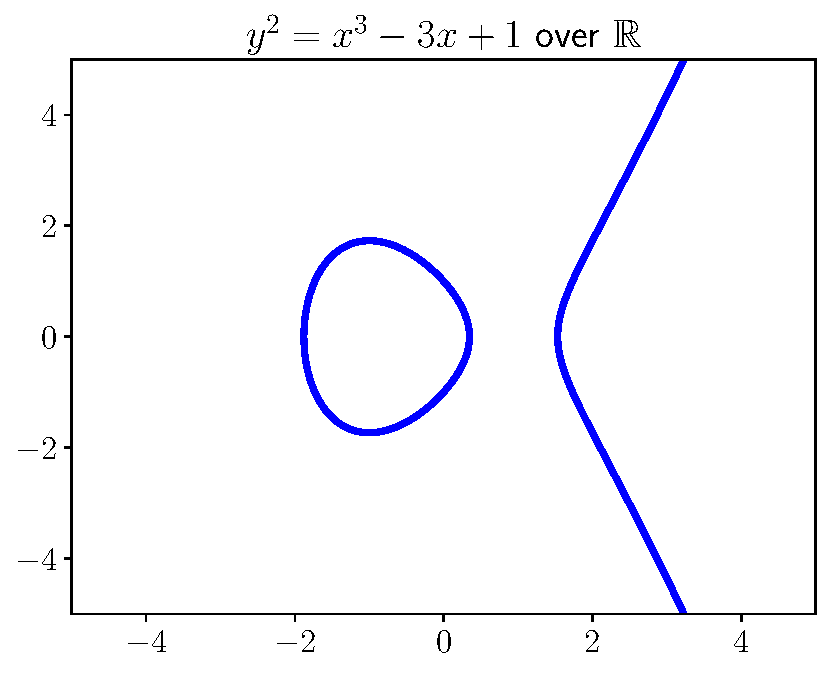
\includegraphics[width=\textwidth]{plots/ec_reals/ec_reals_n3_1.pdf}
    \end{subfigure}
    \begin{subfigure}[t]{0.45\textwidth}
    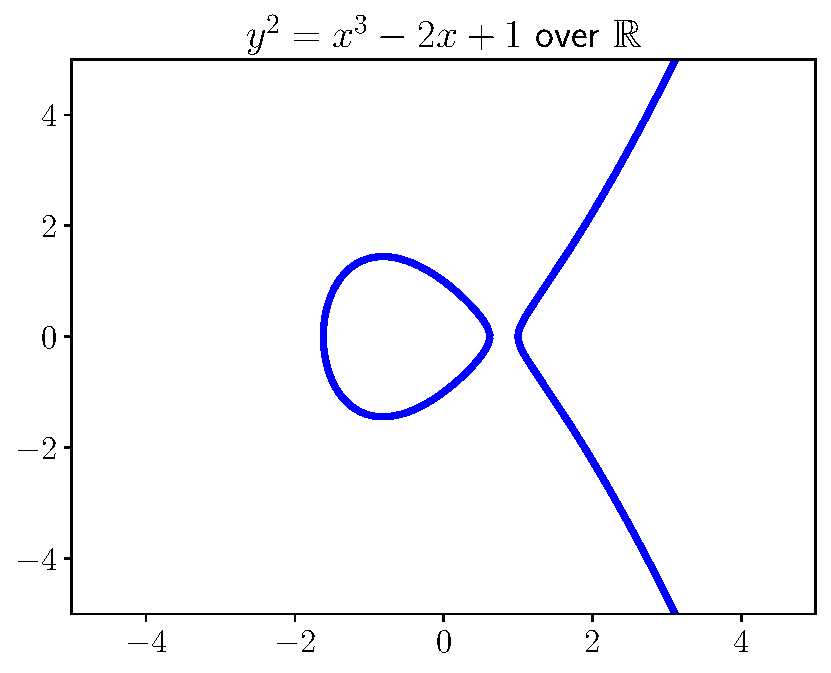
\includegraphics[width=\textwidth]{plots/ec_reals/ec_reals_n2_1.pdf}
    \end{subfigure}

    \begin{subfigure}[t]{0.45\textwidth}
    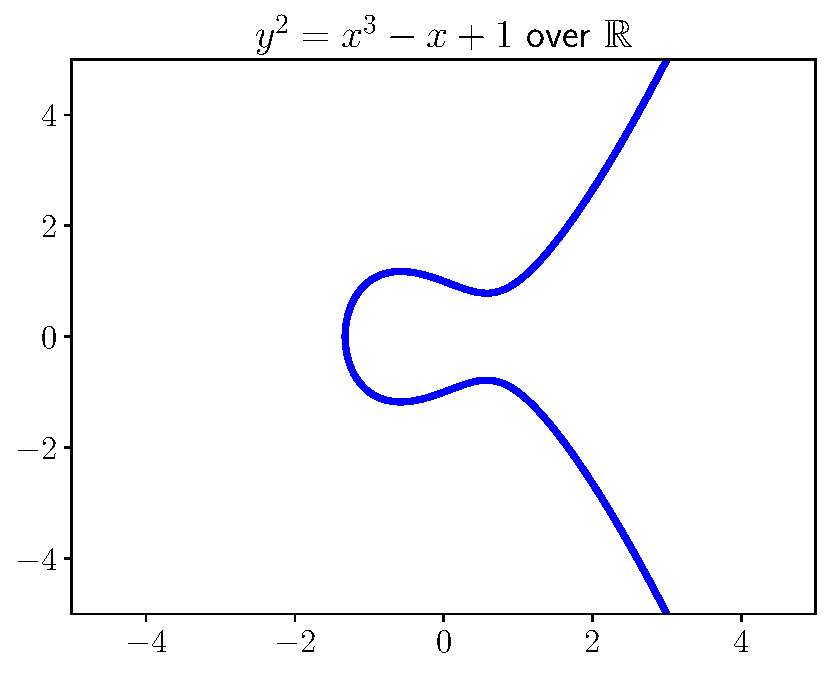
\includegraphics[width=\textwidth]{plots/ec_reals/ec_reals_n1_1.pdf}
    \end{subfigure}
    \begin{subfigure}[t]{0.45\textwidth}
    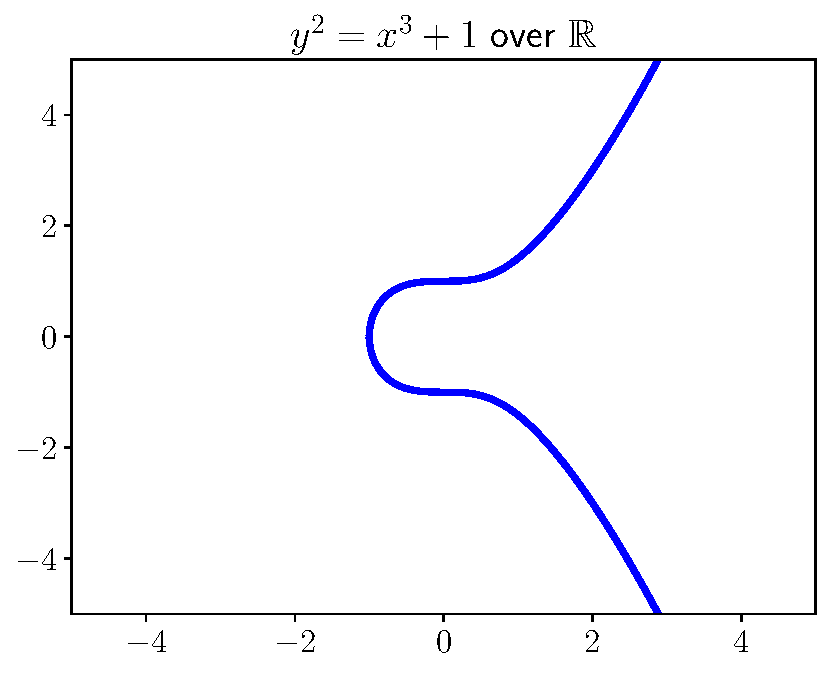
\includegraphics[width=\textwidth]{plots/ec_reals/ec_reals_0_1.pdf}
    \end{subfigure}

    \begin{subfigure}[t]{0.45\textwidth}
    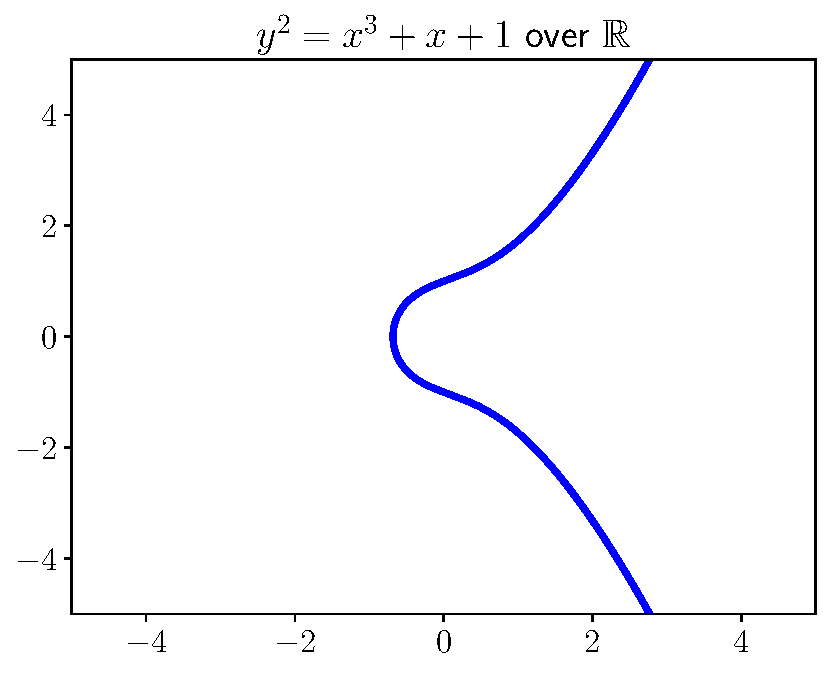
\includegraphics[width=\textwidth]{plots/ec_reals/ec_reals_1_1.pdf}
    \end{subfigure}
    \begin{subfigure}[t]{0.45\textwidth}
    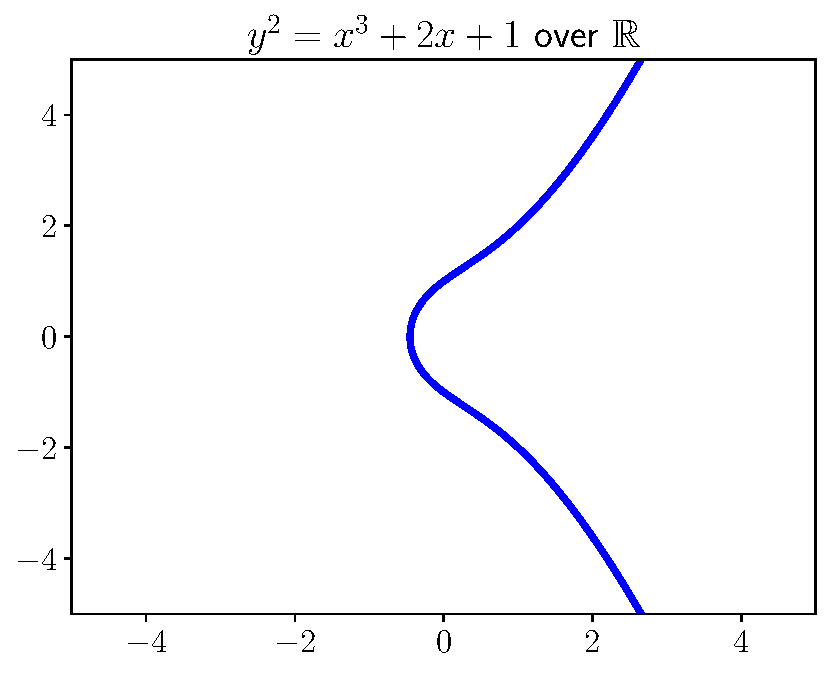
\includegraphics[width=\textwidth]{plots/ec_reals/ec_reals_2_1.pdf}
    \end{subfigure}
    \caption[Plots of elliptic curves over the reals 1]{Here
        are plots of \glspl{elliptic curve} over $\R$.
        The $\parens{x,y}$ points satisfy the equation
        $y^{2} = x^{3} + ax + b$;
        we vary $a$ and hold $b$ constant.}
    \label{fig:ec_real_plots_1}
\end{figure}

\begin{figure}[p]
\centering
    \begin{subfigure}[t]{0.45\textwidth}
    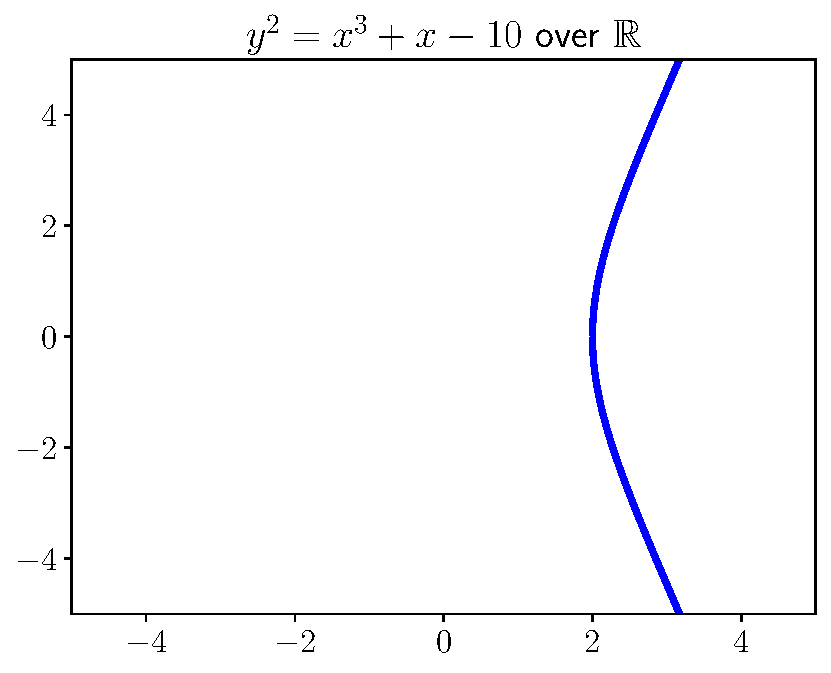
\includegraphics[width=\textwidth]{plots/ec_reals/ec_reals_1_n10.pdf}
    \end{subfigure}
    \begin{subfigure}[t]{0.45\textwidth}
    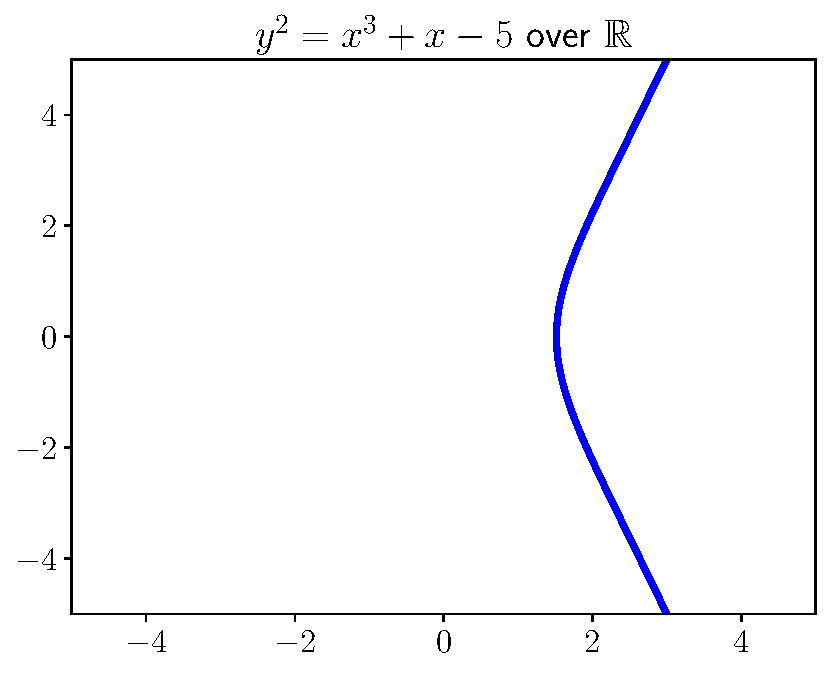
\includegraphics[width=\textwidth]{plots/ec_reals/ec_reals_1_n5.pdf}
    \end{subfigure}

    \begin{subfigure}[t]{0.45\textwidth}
    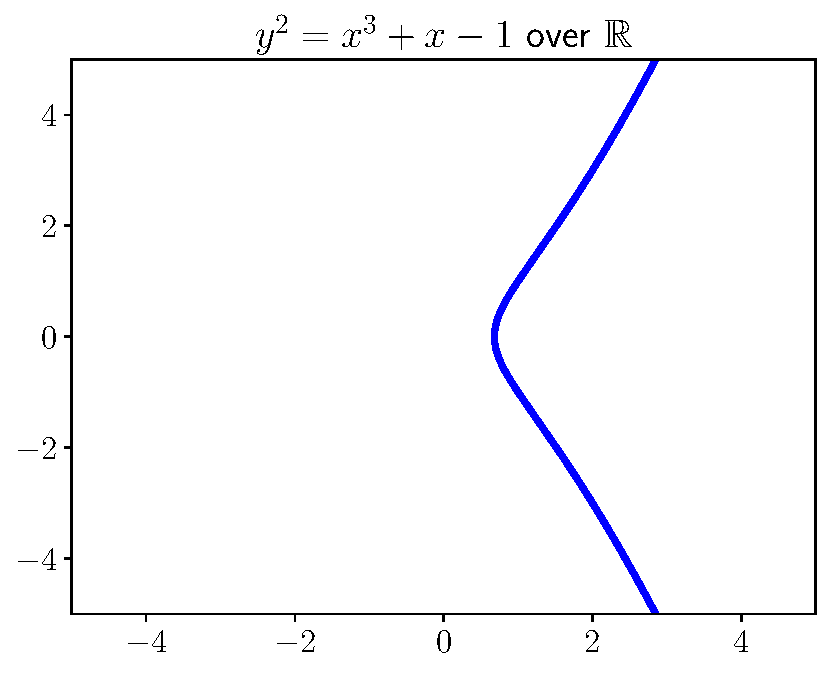
\includegraphics[width=\textwidth]{plots/ec_reals/ec_reals_1_n1.pdf}
    \end{subfigure}
    \begin{subfigure}[t]{0.45\textwidth}
    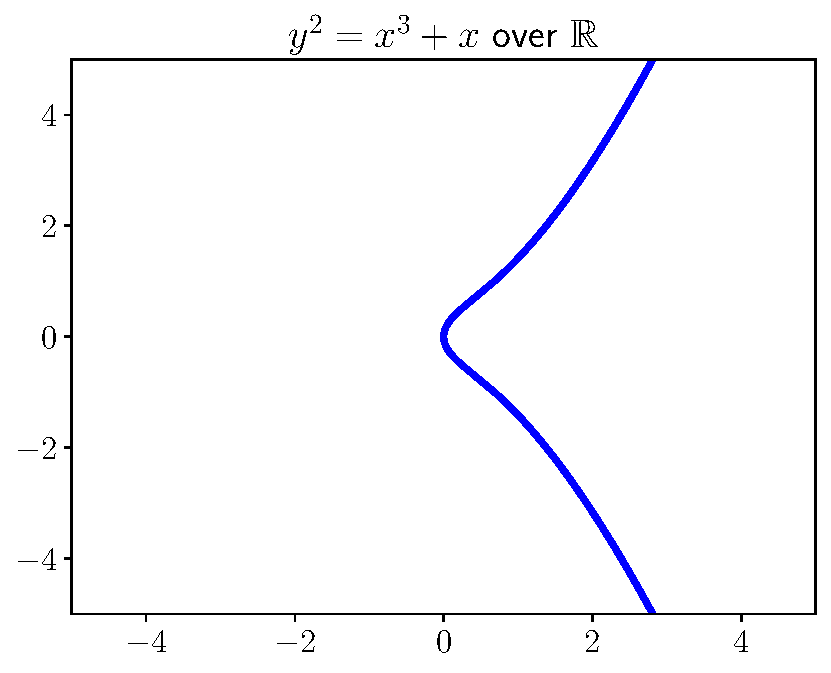
\includegraphics[width=\textwidth]{plots/ec_reals/ec_reals_1_0.pdf}
    \end{subfigure}

    \begin{subfigure}[t]{0.45\textwidth}
    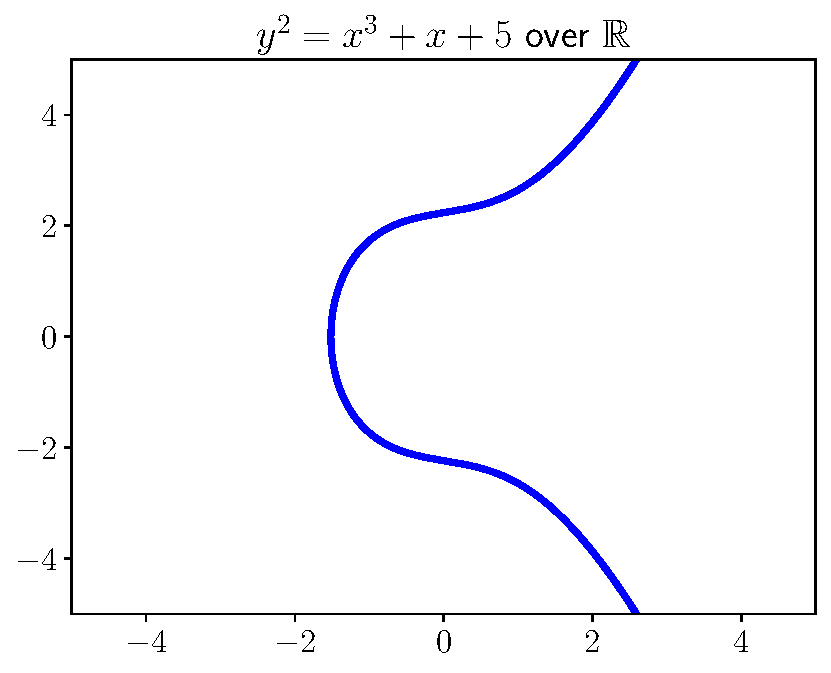
\includegraphics[width=\textwidth]{plots/ec_reals/ec_reals_1_5.pdf}
    \end{subfigure}
    \begin{subfigure}[t]{0.45\textwidth}
    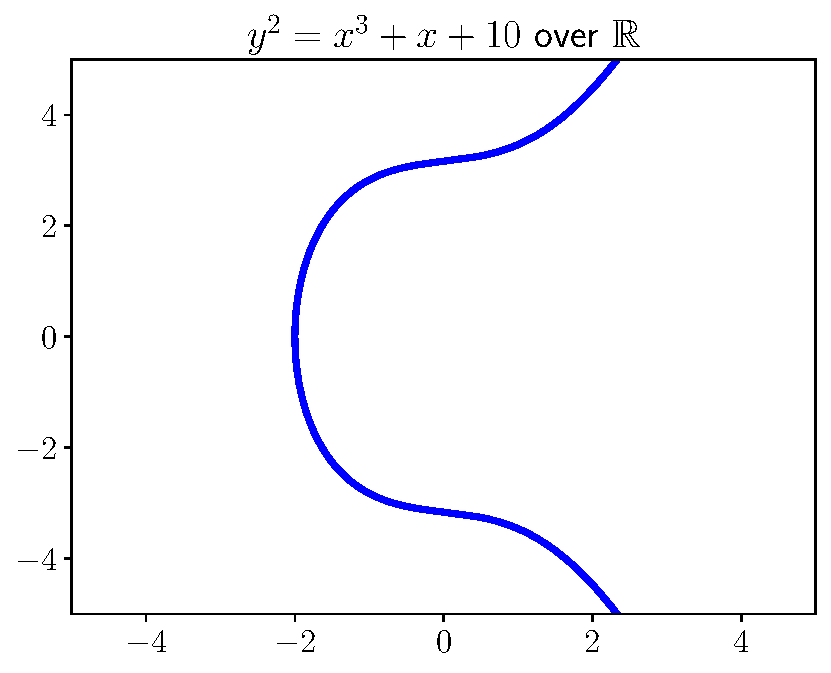
\includegraphics[width=\textwidth]{plots/ec_reals/ec_reals_1_10.pdf}
    \end{subfigure}
    \caption[Plots of elliptic curves over the reals 2]{Here
        are additional plots of \glspl{elliptic curve} over $\R$.
        The $\parens{x,y}$ points satisfy the equation
        $y^{2} = x^{3} + ax + b$;
        we vary $b$ and hold $a$ constant.}
    \label{fig:ec_real_plots_2}
\end{figure}
